% Professional coding-theory logo: codeword + matrix + polynomial
% Standalone TikZ source for presentation/tikzs/logo-codeword-matrix-polynomial.pdf
\documentclass[tikz, border=14pt]{standalone}

\usepackage[T1]{fontenc}
\usepackage[utf8]{inputenc}
\usepackage{amsmath, amssymb}
\usepackage{helvet}
\renewcommand{\familydefault}{\sfdefault}
\usepackage{xcolor}

\usetikzlibrary{
  arrows.meta,
  calc,
  positioning,
  shapes.geometric
}

\definecolor{inkC}{HTML}{101A24}
\definecolor{paperC}{HTML}{F8FBFC}
\definecolor{gridC}{HTML}{DCEAEC}
\definecolor{codeC}{HTML}{008C8C}
\definecolor{codeDarkC}{HTML}{006A70}
\definecolor{matrixC}{HTML}{3155A4}
\definecolor{polyC}{HTML}{B87511}
\definecolor{errC}{HTML}{D33F49}

\begin{document}
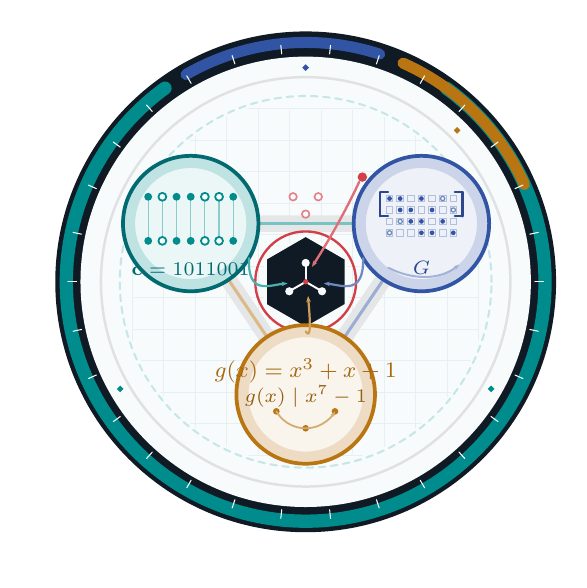
\begin{tikzpicture}[
  x=1cm,
  y=1cm,
  font=\sffamily,
  line cap=round,
  line join=round
]

\def\Rbadge{3.18}
\def\Rinner{2.86}
\coordinate (O) at (0,0);
\coordinate (CW) at (-1.46,0.74);
\coordinate (MX) at (1.47,0.74);
\coordinate (PX) at (0,-1.43);

% Badge and dominant coding ring.
\fill[inkC] (O) circle (\Rbadge);
\draw[codeC, line width=4.8pt] (126:3.04) arc[start angle=126, end angle=414, radius=3.04];
\draw[matrixC, line width=4.0pt] (72:3.04) arc[start angle=72, end angle=120, radius=3.04];
\draw[polyC, line width=4.0pt] (24:3.04) arc[start angle=24, end angle=66, radius=3.04];
\fill[paperC] (O) circle (\Rinner);
\draw[inkC!13, line width=0.90pt] (O) circle (2.60);
\draw[codeC!22, line width=0.75pt, dash pattern=on 2.4pt off 2pt] (O) circle (2.36);

\foreach \ang in {0,12,...,348}{
  \draw[paperC!56, line width=0.38pt] (\ang:2.91) -- (\ang:3.02);
}

% Faint vector-space grid.
\begin{scope}
  \clip (O) circle (2.32);
  \foreach \x in {-2.2,-1.8,...,2.2}{
    \draw[gridC!70, line width=0.34pt] (\x,-2.18) -- (\x,2.18);
  }
  \foreach \y in {-2.2,-1.8,...,2.2}{
    \draw[gridC!70, line width=0.34pt] (-2.18,\y) -- (2.18,\y);
  }
\end{scope}

% Three coding-theory objects connected as encoder algebra.
\draw[inkC!11, line width=6.0pt] (CW) -- (MX) -- (PX) -- cycle;
\draw[codeC!52, line width=1.10pt] (CW) -- (MX);
\draw[matrixC!48, line width=1.10pt] (MX) -- (PX);
\draw[polyC!50, line width=1.10pt] (PX) -- (CW);

% Central encoder core.
\node[
  regular polygon,
  regular polygon sides=6,
  rotate=30,
  minimum size=1.18cm,
  inner sep=0pt,
  fill=inkC,
  draw=paperC,
  line width=1.0pt
] at (O) {};
\draw[errC, line width=0.85pt] (O) circle (0.64);
\foreach \ang in {90,210,330}{
  \fill[paperC] (\ang:0.24) circle (0.052);
  \draw[paperC!78, line width=0.70pt] (O) -- (\ang:0.24);
}
\fill[errC] (O) circle (0.034);

% Codeword medallion.
\begin{scope}[shift={(CW)}]
  \fill[paperC] (0,0) circle (0.86);
  \fill[codeC!8] (0,0) circle (0.76);
  \draw[codeC!25, line width=4.2pt] (0,0) circle (0.78);
  \draw[codeDarkC, line width=1.35pt] (0,0) circle (0.86);

  \foreach \i/\bit in {0/1,1/0,2/1,3/1,4/0,5/0,6/1}{
    \pgfmathsetmacro{\xx}{-0.54+0.18*\i}
    \draw[codeC!45, line width=0.42pt] (\xx,-0.18) -- (\xx,0.30);
    \ifnum\bit=1
      \fill[codeC] (\xx,0.34) circle (0.050);
      \fill[codeC] (\xx,-0.22) circle (0.050);
    \else
      \fill[paperC] (\xx,0.34) circle (0.050);
      \draw[codeC, line width=0.65pt] (\xx,0.34) circle (0.050);
      \fill[paperC] (\xx,-0.22) circle (0.050);
      \draw[codeC, line width=0.65pt] (\xx,-0.22) circle (0.050);
    \fi
  }

  \node[codeDarkC, font=\scriptsize\bfseries] at (0,-0.58)
    {$\mathbf c=1011001$};
\end{scope}

% Matrix medallion.
\begin{scope}[shift={(MX)}]
  \fill[paperC] (0,0) circle (0.86);
  \fill[matrixC!8] (0,0) circle (0.76);
  \draw[matrixC!25, line width=4.2pt] (0,0) circle (0.78);
  \draw[matrixC, line width=1.35pt] (0,0) circle (0.86);

  \pgfmathsetmacro{\mxs}{0.135}
  \pgfmathsetmacro{\mys}{0.145}
  \pgfmathsetmacro{\mxo}{-3.0*\mxs}
  \pgfmathsetmacro{\myo}{1.5*\mys+0.10}

  \foreach \col in {0,1,2,3,4,5,6}{
    \foreach \row in {0,1,2,3}{
      \draw[matrixC!38, line width=0.34pt]
        ({\mxo+\col*\mxs-0.042},{\myo-\row*\mys-0.042}) rectangle
        ({\mxo+\col*\mxs+0.042},{\myo-\row*\mys+0.042});
    }
  }
  \foreach \col/\row in {
    0/0,1/0,3/0,
    1/1,2/1,4/1,
    2/2,3/2,5/2,
    3/3,4/3,6/3
  }{
    \fill[matrixC] ({\mxo+\col*\mxs},{\myo-\row*\mys}) circle (0.030);
  }
  \foreach \col/\row in {0/3,1/2,5/0,6/1}{
    \fill[paperC] ({\mxo+\col*\mxs},{\myo-\row*\mys}) circle (0.027);
    \draw[matrixC!70, line width=0.45pt]
      ({\mxo+\col*\mxs},{\myo-\row*\mys}) circle (0.027);
  }

  \pgfmathsetmacro{\mbrx}{3.55*\mxs}
  \pgfmathsetmacro{\mbry}{2.05*\mys}
  \draw[matrixC!85!black, line width=0.88pt]
    ({-\mbrx-0.045},{\myo-\mbry+0.5*\mys}) -- ({-\mbrx-0.045},{\myo+\mbry-1.5*\mys})
    ({-\mbrx-0.045},{\myo+\mbry-1.5*\mys}) -- ({-\mbrx+0.055},{\myo+\mbry-1.5*\mys})
    ({-\mbrx-0.045},{\myo-\mbry+0.5*\mys}) -- ({-\mbrx+0.055},{\myo-\mbry+0.5*\mys});
  \draw[matrixC!85!black, line width=0.88pt]
    ({\mbrx+0.045},{\myo-\mbry+0.5*\mys}) -- ({\mbrx+0.045},{\myo+\mbry-1.5*\mys})
    ({\mbrx+0.045},{\myo+\mbry-1.5*\mys}) -- ({\mbrx-0.055},{\myo+\mbry-1.5*\mys})
    ({\mbrx+0.045},{\myo-\mbry+0.5*\mys}) -- ({\mbrx-0.055},{\myo-\mbry+0.5*\mys});

  \node[matrixC!85!black, font=\scriptsize\bfseries] at (0,-0.56) {$G$};

  \draw[matrixC!45, line width=0.70pt, -{Stealth[length=2.0pt]}]
    (-0.42,-0.56) .. controls (-0.12,-0.72) and (0.24,-0.72) .. (0.48,-0.52);
\end{scope}

% Polynomial medallion.
\begin{scope}[shift={(PX)}]
  \fill[paperC] (0,0) circle (0.88);
  \fill[polyC!8] (0,0) circle (0.78);
  \draw[polyC!25, line width=4.2pt] (0,0) circle (0.80);
  \draw[polyC, line width=1.35pt] (0,0) circle (0.88);

  \node[polyC!90!black, font=\footnotesize\bfseries] at (0,0.30)
    {$g(x)=x^3+x+1$};
  \node[polyC!80!black, font=\scriptsize] at (0,-0.03)
    {$g(x)\mid x^7-1$};

  \foreach \ang in {210,270,330}{
    \fill[polyC] (\ang:0.43) circle (0.042);
  }
  \draw[polyC!60, line width=0.65pt, -{Stealth[length=2.0pt]}]
    (210:0.43) arc[start angle=210, end angle=330, radius=0.43];
\end{scope}

% Encoder arrows: message to codeword, matrix to codeword, polynomial to cyclic code.
\draw[codeC!70, line width=0.80pt, -{Stealth[length=2.2pt]}]
  ($(CW)+(0.74,-0.44)$) .. controls (-0.74,-0.18) and (-0.46,-0.04) .. (-0.23,-0.02);
\draw[matrixC!70, line width=0.80pt, -{Stealth[length=2.2pt]}]
  ($(MX)+(-0.74,-0.44)$) .. controls (0.74,-0.18) and (0.46,-0.04) .. (0.23,-0.02);
\draw[polyC!70, line width=0.80pt, -{Stealth[length=2.2pt]}]
  ($(PX)+(0,0.80)$) .. controls (0.08,-0.76) and (0.05,-0.42) .. (0.03,-0.18);

% Error and syndrome hint.
\fill[errC] (0.72,1.33) circle (0.060);
\draw[errC!75, line width=0.85pt, -{Stealth[length=2.2pt]}]
  (0.68,1.27) .. controls (0.47,0.82) and (0.24,0.44) .. (0.08,0.19);
\foreach \p in {(-0.16,1.08),(0.16,1.08),(0,0.86)}{
  \fill[paperC] \p circle (0.048);
  \draw[errC!65, line width=0.60pt] \p circle (0.048);
}

% Small rim separators.
\foreach \ang/\C in {90/matrixC, 210/codeC, 330/codeC, 45/polyC}{
  \node[
    regular polygon,
    regular polygon sides=4,
    rotate=45,
    fill=\C,
    minimum size=0.085cm,
    inner sep=0pt
  ] at (\ang:2.72) {};
}

\end{tikzpicture}
\end{document}
